% Options for packages loaded elsewhere
\PassOptionsToPackage{unicode}{hyperref}
\PassOptionsToPackage{hyphens}{url}
%
\documentclass[
]{article}
\usepackage{lmodern}
\usepackage{amssymb,amsmath}
\usepackage{ifxetex,ifluatex}
\ifnum 0\ifxetex 1\fi\ifluatex 1\fi=0 % if pdftex
  \usepackage[T1]{fontenc}
  \usepackage[utf8]{inputenc}
  \usepackage{textcomp} % provide euro and other symbols
\else % if luatex or xetex
  \usepackage{unicode-math}
  \defaultfontfeatures{Scale=MatchLowercase}
  \defaultfontfeatures[\rmfamily]{Ligatures=TeX,Scale=1}
\fi
% Use upquote if available, for straight quotes in verbatim environments
\IfFileExists{upquote.sty}{\usepackage{upquote}}{}
\IfFileExists{microtype.sty}{% use microtype if available
  \usepackage[]{microtype}
  \UseMicrotypeSet[protrusion]{basicmath} % disable protrusion for tt fonts
}{}
\makeatletter
\@ifundefined{KOMAClassName}{% if non-KOMA class
  \IfFileExists{parskip.sty}{%
    \usepackage{parskip}
  }{% else
    \setlength{\parindent}{0pt}
    \setlength{\parskip}{6pt plus 2pt minus 1pt}}
}{% if KOMA class
  \KOMAoptions{parskip=half}}
\makeatother
\usepackage{xcolor}
\IfFileExists{xurl.sty}{\usepackage{xurl}}{} % add URL line breaks if available
\IfFileExists{bookmark.sty}{\usepackage{bookmark}}{\usepackage{hyperref}}
\hypersetup{
  pdftitle={Framanburdur},
  hidelinks,
  pdfcreator={LaTeX via pandoc}}
\urlstyle{same} % disable monospaced font for URLs
\usepackage[margin=1in]{geometry}
\usepackage{color}
\usepackage{fancyvrb}
\newcommand{\VerbBar}{|}
\newcommand{\VERB}{\Verb[commandchars=\\\{\}]}
\DefineVerbatimEnvironment{Highlighting}{Verbatim}{commandchars=\\\{\}}
% Add ',fontsize=\small' for more characters per line
\usepackage{framed}
\definecolor{shadecolor}{RGB}{248,248,248}
\newenvironment{Shaded}{\begin{snugshade}}{\end{snugshade}}
\newcommand{\AlertTok}[1]{\textcolor[rgb]{0.94,0.16,0.16}{#1}}
\newcommand{\AnnotationTok}[1]{\textcolor[rgb]{0.56,0.35,0.01}{\textbf{\textit{#1}}}}
\newcommand{\AttributeTok}[1]{\textcolor[rgb]{0.77,0.63,0.00}{#1}}
\newcommand{\BaseNTok}[1]{\textcolor[rgb]{0.00,0.00,0.81}{#1}}
\newcommand{\BuiltInTok}[1]{#1}
\newcommand{\CharTok}[1]{\textcolor[rgb]{0.31,0.60,0.02}{#1}}
\newcommand{\CommentTok}[1]{\textcolor[rgb]{0.56,0.35,0.01}{\textit{#1}}}
\newcommand{\CommentVarTok}[1]{\textcolor[rgb]{0.56,0.35,0.01}{\textbf{\textit{#1}}}}
\newcommand{\ConstantTok}[1]{\textcolor[rgb]{0.00,0.00,0.00}{#1}}
\newcommand{\ControlFlowTok}[1]{\textcolor[rgb]{0.13,0.29,0.53}{\textbf{#1}}}
\newcommand{\DataTypeTok}[1]{\textcolor[rgb]{0.13,0.29,0.53}{#1}}
\newcommand{\DecValTok}[1]{\textcolor[rgb]{0.00,0.00,0.81}{#1}}
\newcommand{\DocumentationTok}[1]{\textcolor[rgb]{0.56,0.35,0.01}{\textbf{\textit{#1}}}}
\newcommand{\ErrorTok}[1]{\textcolor[rgb]{0.64,0.00,0.00}{\textbf{#1}}}
\newcommand{\ExtensionTok}[1]{#1}
\newcommand{\FloatTok}[1]{\textcolor[rgb]{0.00,0.00,0.81}{#1}}
\newcommand{\FunctionTok}[1]{\textcolor[rgb]{0.00,0.00,0.00}{#1}}
\newcommand{\ImportTok}[1]{#1}
\newcommand{\InformationTok}[1]{\textcolor[rgb]{0.56,0.35,0.01}{\textbf{\textit{#1}}}}
\newcommand{\KeywordTok}[1]{\textcolor[rgb]{0.13,0.29,0.53}{\textbf{#1}}}
\newcommand{\NormalTok}[1]{#1}
\newcommand{\OperatorTok}[1]{\textcolor[rgb]{0.81,0.36,0.00}{\textbf{#1}}}
\newcommand{\OtherTok}[1]{\textcolor[rgb]{0.56,0.35,0.01}{#1}}
\newcommand{\PreprocessorTok}[1]{\textcolor[rgb]{0.56,0.35,0.01}{\textit{#1}}}
\newcommand{\RegionMarkerTok}[1]{#1}
\newcommand{\SpecialCharTok}[1]{\textcolor[rgb]{0.00,0.00,0.00}{#1}}
\newcommand{\SpecialStringTok}[1]{\textcolor[rgb]{0.31,0.60,0.02}{#1}}
\newcommand{\StringTok}[1]{\textcolor[rgb]{0.31,0.60,0.02}{#1}}
\newcommand{\VariableTok}[1]{\textcolor[rgb]{0.00,0.00,0.00}{#1}}
\newcommand{\VerbatimStringTok}[1]{\textcolor[rgb]{0.31,0.60,0.02}{#1}}
\newcommand{\WarningTok}[1]{\textcolor[rgb]{0.56,0.35,0.01}{\textbf{\textit{#1}}}}
\usepackage{longtable,booktabs}
% Correct order of tables after \paragraph or \subparagraph
\usepackage{etoolbox}
\makeatletter
\patchcmd\longtable{\par}{\if@noskipsec\mbox{}\fi\par}{}{}
\makeatother
% Allow footnotes in longtable head/foot
\IfFileExists{footnotehyper.sty}{\usepackage{footnotehyper}}{\usepackage{footnote}}
\makesavenoteenv{longtable}
\usepackage{graphicx,grffile}
\makeatletter
\def\maxwidth{\ifdim\Gin@nat@width>\linewidth\linewidth\else\Gin@nat@width\fi}
\def\maxheight{\ifdim\Gin@nat@height>\textheight\textheight\else\Gin@nat@height\fi}
\makeatother
% Scale images if necessary, so that they will not overflow the page
% margins by default, and it is still possible to overwrite the defaults
% using explicit options in \includegraphics[width, height, ...]{}
\setkeys{Gin}{width=\maxwidth,height=\maxheight,keepaspectratio}
% Set default figure placement to htbp
\makeatletter
\def\fps@figure{htbp}
\makeatother
\setlength{\emergencystretch}{3em} % prevent overfull lines
\providecommand{\tightlist}{%
  \setlength{\itemsep}{0pt}\setlength{\parskip}{0pt}}
\setcounter{secnumdepth}{5}

\title{Framanburdur}
\author{}
\date{\vspace{-2.5em}}

\begin{document}
\maketitle

{
\setcounter{tocdepth}{2}
\tableofcontents
}
\hypertarget{gagna-innlestur}{%
\subsection{Gagna Innlestur}\label{gagna-innlestur}}

Lesið er inn gögninn

\begin{Shaded}
\begin{Highlighting}[]
\NormalTok{hashAnswer <-}\StringTok{ }\KeywordTok{read.csv}\NormalTok{(}\StringTok{'Data/hashAnswer4.csv'}\NormalTok{)}
\NormalTok{hashAnswer <-}\StringTok{ }\NormalTok{hashAnswer }\OperatorTok\StringTok{ }\KeywordTok{subset}\NormalTok{(}\DataTypeTok{select=}\OperatorTok{-}\KeywordTok{c}\NormalTok{(X))}
\NormalTok{hashAnswer}\OperatorTok{$}\NormalTok{hsta <-}\StringTok{ }\NormalTok{hashAnswer}\OperatorTok{$}\NormalTok{hsta}\OperatorTok\KeywordTok{as.character}\NormalTok{()}
\NormalTok{hashAnswer}\OperatorTok{$}\NormalTok{lectureId <-}\StringTok{ }\NormalTok{hashAnswer}\OperatorTok{$}\NormalTok{lectureId }\OperatorTok\StringTok{ }\KeywordTok{as.factor}\NormalTok{()}
\NormalTok{hashAnswer}\OperatorTok{$}\NormalTok{studentId <-}\StringTok{ }\NormalTok{hashAnswer}\OperatorTok{$}\NormalTok{studentId }\OperatorTok\StringTok{ }\KeywordTok{as.factor}\NormalTok{()}
\end{Highlighting}
\end{Shaded}

Þetta eru tutor-web gögn fyrir lík og töl í vormisseri 2020. \textbackslash{}

\begin{Shaded}
\begin{Highlighting}[]
\KeywordTok{glimpse}\NormalTok{(hashAnswer)}
\end{Highlighting}
\end{Shaded}

\begin{verbatim}
## Rows: 115,002
## Columns: 11
## $ timeStart  <chr> "2020-01-15 10:24:32", "2020-01-15 10:26:20", "2020-01-1...
## $ lectureId  <fct> 3082, 3082, 3082, 3082, 3082, 3082, 3082, 3082, 3082, 30...
## $ studentId  <fct> 1, 1, 1, 1, 1, 18788, 18788, 18788, 18788, 18788, 18788,...
## $ questionId <int> 45591, 44899, 45647, 45647, 45647, 44920, 45021, 45480, ...
## $ correct    <int> 0, 1, 0, 0, 0, 1, 0, 1, 1, 0, 0, 1, 1, 0, 0, 0, 0, 0, 1,...
## $ hash       <chr> "d3a978206c877eee8627a29c7a94238d8339d66fc4be460d9e6b6cb...
## $ fsfat      <int> 0, 1, 2, 2, 2, 0, 1, 2, 3, 4, 5, 6, 7, 8, 9, 9, 9, 10, 1...
## $ fsvfat     <int> 0, 1, 2, 3, 4, 0, 1, 2, 3, 4, 5, 5, 6, 7, 8, 9, 10, 11, ...
## $ fsvfatu    <int> 0, 1, 2, 2, 2, 0, 1, 2, 3, 4, 5, 5, 6, 7, 8, 8, 8, 11, 1...
## $ hsta       <chr> "0", "0", "0", "0", "0", "0", "0", "0", "0", "0", "0", "...
## $ timeDif    <int> NA, NA, NA, NA, NA, NA, NA, NA, NA, NA, NA, 254, NA, NA,...
\end{verbatim}

Gögninn innihalda factor breyturnar lectureId, studentId og questionId. Sem eru einkenningar fyrirlesturinns, nemendans og spurningarnar. Næst inniheldur það correct sem er binary breyta fyrir því hvort fengið var rétt eða rangt svar. Hash er einkvæm tenging fyrir hvert svar. fsfat er ``Fjöldi spurninga fram að þessu'' sem telur upp hve margar spurningar nemandinn hefur svarað hingað til í þessum fyrirlestri. fsvfat er ``Fjöldi svara fram að þessu'' sem telur upp hve ný svör nemandinn hefur séð að þessum punkti. fsvfatu ``Fjöldi svara fram að þessu uppfært'' þetta er temporary nafn sem kemur fyrir fsvfat nema þegar AOTA+ spurning kemur þá heldur það sama fsvfat fyrir þá spurningu, telst samt venjulega annars. hsta ``hef séð þetta áður'' þetta er 0 eða 1 sem segir til hvort nemandinn hefur séð svarið áður eða ekki. Að lokum er timeDif sem segir til hve margar sekúndur hafa varið séðan þetta svar kom seinast. \textbackslash{}
\textbackslash{}
Fyrsta sem ég gerði var að skoða aðeins einföld logistic regression föll, skipt upp eftir því hve margar spurningar, semsagt fsfat ég leifi að svara. Þá fyrir fsfat og fyrir fsvfat.
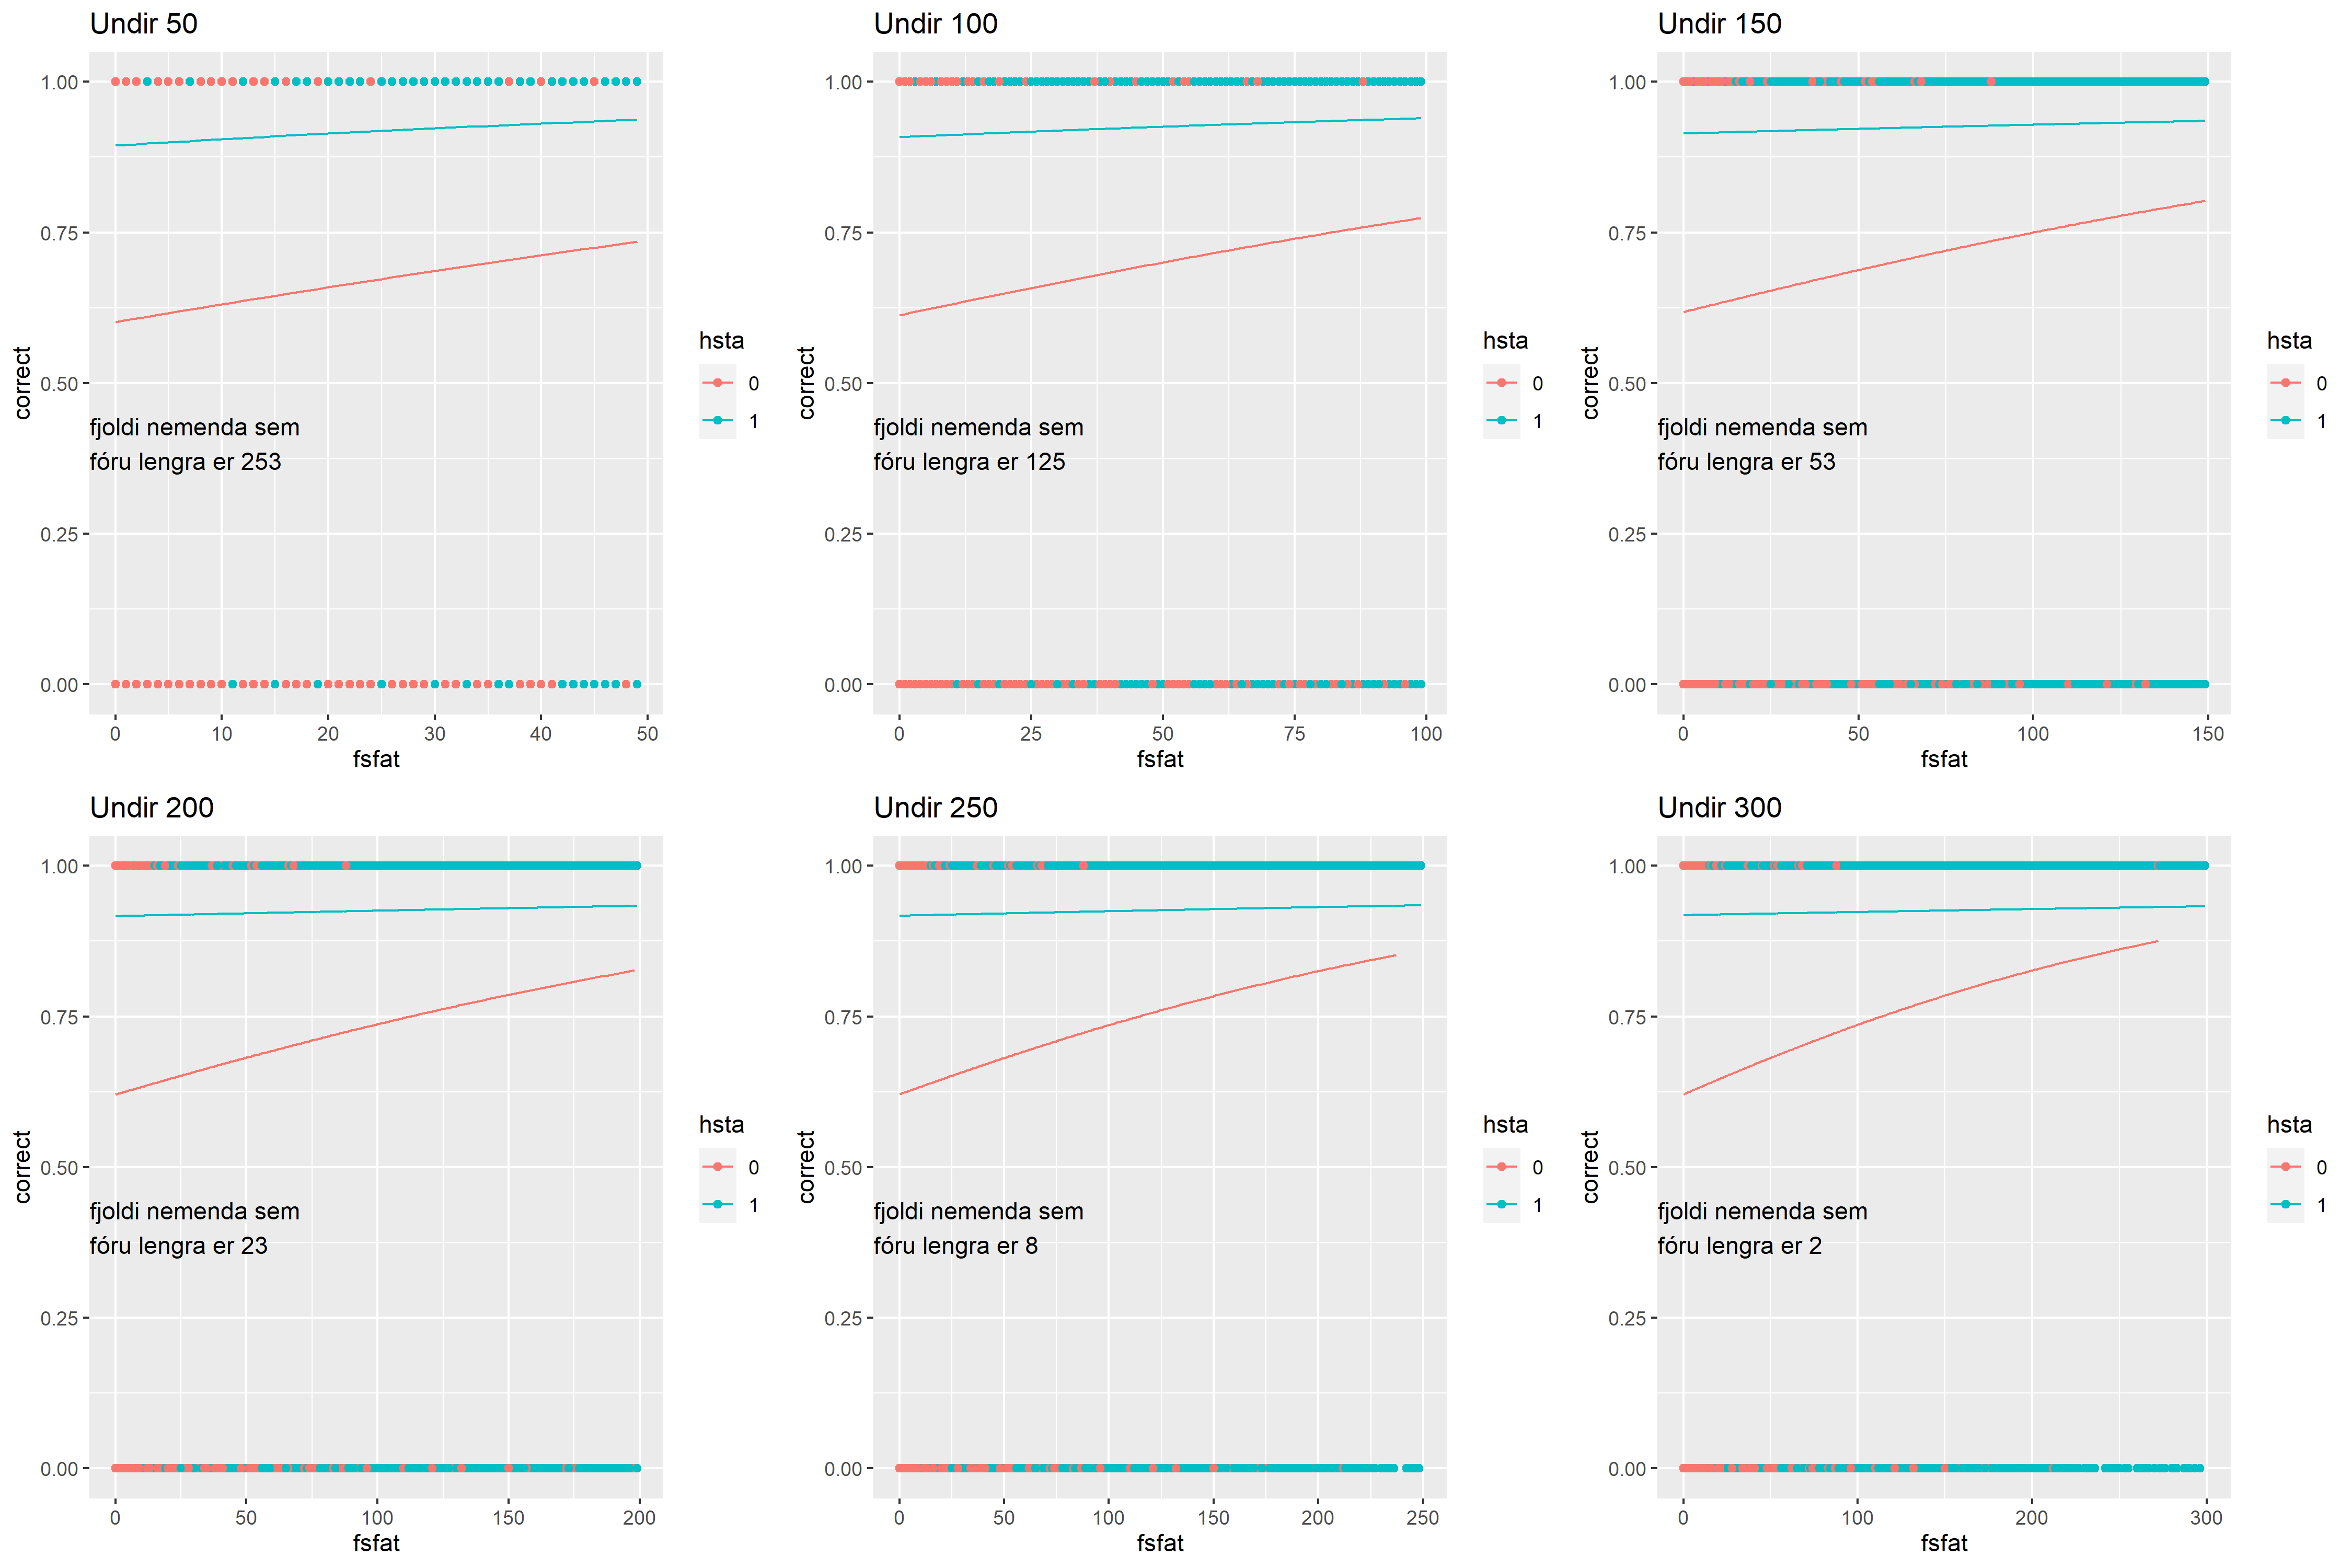
\includegraphics{Img/plot1.png}

\end{document}
